%%%%%%%%%%%%%%%%%%%%%%%%%%%%%%%%%%%%%%%%%
% Beamer Presentation
% LaTeX Template
% Version 1.0 (10/11/12)
%
% This template has been downloaded from:
% http://www.LaTeXTemplates.com
%
% License:
% CC BY-NC-SA 3.0 (http://creativecommons.org/licenses/by-nc-sa/3.0/)
%
%%%%%%%%%%%%%%%%%%%%%%%%%%%%%%%%%%%%%%%%%

%----------------------------------------------------------------------------------------
%	PACKAGES AND THEMES
%----------------------------------------------------------------------------------------

\documentclass{beamer}

\mode<presentation> {

% The Beamer class comes with a number of default slide themes
% which change the colors and layouts of slides. Below this is a list
% of all the themes, uncomment each in turn to see what they look like.

%\usetheme{default}
%\usetheme{AnnArbor}
%\usetheme{Antibes}
%\usetheme{Bergen}
%\usetheme{Berkeley}
%\usetheme{Berlin}
%\usetheme{Boadilla}
%\usetheme{CambridgeUS}
%\usetheme{Copenhagen}
%\usetheme{Darmstadt}
%\usetheme{Dresden}
%\usetheme{Frankfurt}
%\usetheme{Goettingen}
%\usetheme{Hannover}
%\usetheme{Ilmenau}
%\usetheme{JuanLesPins}
%\usetheme{Luebeck}
\usetheme{Madrid}
%\usetheme{Malmoe}
%\usetheme{Marburg}
%\usetheme{Montpellier}
%\usetheme{PaloAlto}
%\usetheme{Pittsburgh}
%\usetheme{Rochester}
%\usetheme{Singapore}
%\usetheme{Szeged}
%\usetheme{Warsaw}

% As well as themes, the Beamer class has a number of color themes
% for any slide theme. Uncomment each of these in turn to see how it
% changes the colors of your current slide theme.

%\usecolortheme{albatross}
%\usecolortheme{beaver}
%\usecolortheme{beetle}
%\usecolortheme{crane}
%\usecolortheme{dolphin}
%\usecolortheme{dove}
%\usecolortheme{fly}
%\usecolortheme{lily}
%\usecolortheme{orchid}
%\usecolortheme{rose}
%\usecolortheme{seagull}
%\usecolortheme{seahorse}
%\usecolortheme{whale}
%\usecolortheme{wolverine}

%\setbeamertemplate{footline} % To remove the footer line in all slides uncomment this line
%\setbeamertemplate{footline}[page number] % To replace the footer line in all slides with a simple slide count uncomment this line

%\setbeamertemplate{navigation symbols}{} % To remove the navigation symbols from the bottom of all slides uncomment this line
}

\usepackage[export]{adjustbox}
\usepackage{graphicx} % Allows including images
\usepackage{booktabs} % Allows the use of \toprule, \midrule and \bottomrule in tables
\graphicspath{ {./figures/} }

%----------------------------------------------------------------------------------------
%	TITLE PAGE
%----------------------------------------------------------------------------------------

\title[ESS-NW/CAR]{ESS-NW/CAR } % The short title appears at the bottom of every slide, the full title is only on the title page

\author{ Leon Fernandez, Jonas Ekman, Fredrik Hyyrynen, Jacob Kimblad, Yini Gao and  Yifan Ruan} % Your name
\institute[KTH] % Your institution as it will appear on the bottom of every slide, may be shorthand to save space
{
MF2063 \\ % Your institution for the title page
\medskip

}
\date{\today} % Date, can be changed to a custom date

\begin{document}

\begin{frame}
\titlepage % Print the title page as the first slide
\end{frame}

\begin{frame}
\frametitle{Overview} % Table of contents slide, comment this block out to remove it
\tableofcontents % Throughout your presentation, if you choose to use \section{} and \subsection{} commands, these will automatically be printed on this slide as an overview of your presentation
\end{frame}

%----------------------------------------------------------------------------------------
%	PRESENTATION SLIDES
%----------------------------------------------------------------------------------------

%------------------------------------------------
\section{Introduction} 
    
\begin{frame}{Introduction}
    \begin{itemize}
        \item Autonomous Driving (AD) and Advandced Driving Assistance Systems (ADAS)
        \item Communication in self driving cars
        \begin{itemize}
            \item CAN
            \item LIN
            \item FlexRay
            \item Ethernet
        \end{itemize}
        \item Intelligent system monitoring
        \begin{itemize}
            \item Startup
            \item Fault detection
            \item Network statistics
        \end{itemize}
        \item Adaptation services
        \begin{itemize}
            \item Failsafe
            \item Network reconfiguration
        \end{itemize}

    \end{itemize}
\end{frame}


%------------------------------------------------

\section{Network}
\subsection{SDN}
\begin{frame}{Network}
    \begin{itemize}
        \item Software defined Network (SDN)
    \end{itemize}
    \begin{figure}
        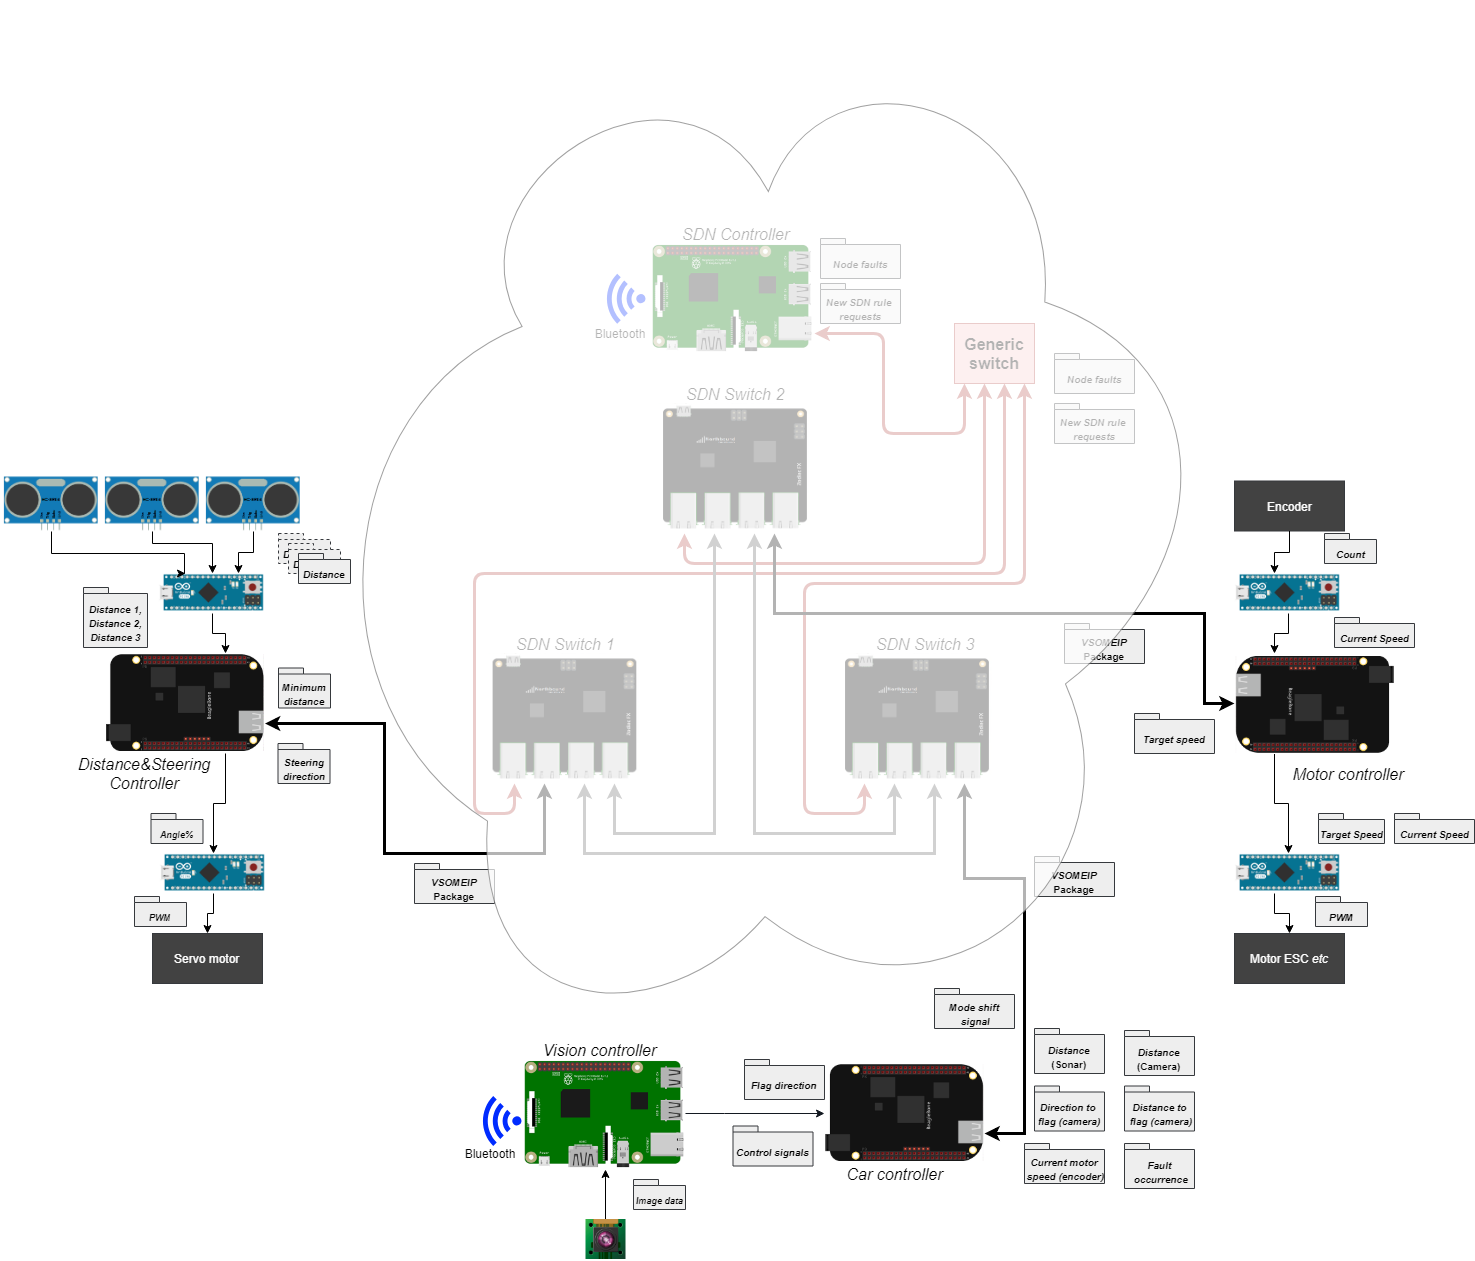
\includegraphics[width=0.6\linewidth]{network.png}
        \caption{Network}
    \end{figure}
\end{frame}



\begin{frame}{SDN}
    \begin{itemize}
        \item Move the intelligence from the switches to a controller
        \item The controller gather information from the switches
        \item The controller decides how the traffic should be send in the network
        \item Scalable
        \item Ryu controller is the SDN frame work we used, python based and well documented.          
    \end{itemize}
    
\end{frame}{}

\subsection{VSome/IP}
\begin{frame}{VSOME/IP}
    
\end{frame}
%------------------------------------------------

\section{Control and sensors }
\subsection{Sensors}

\begin{frame}{Sensors}
    \begin{itemize}
     \item Ultrasonic sensor
    \begin{figure}
        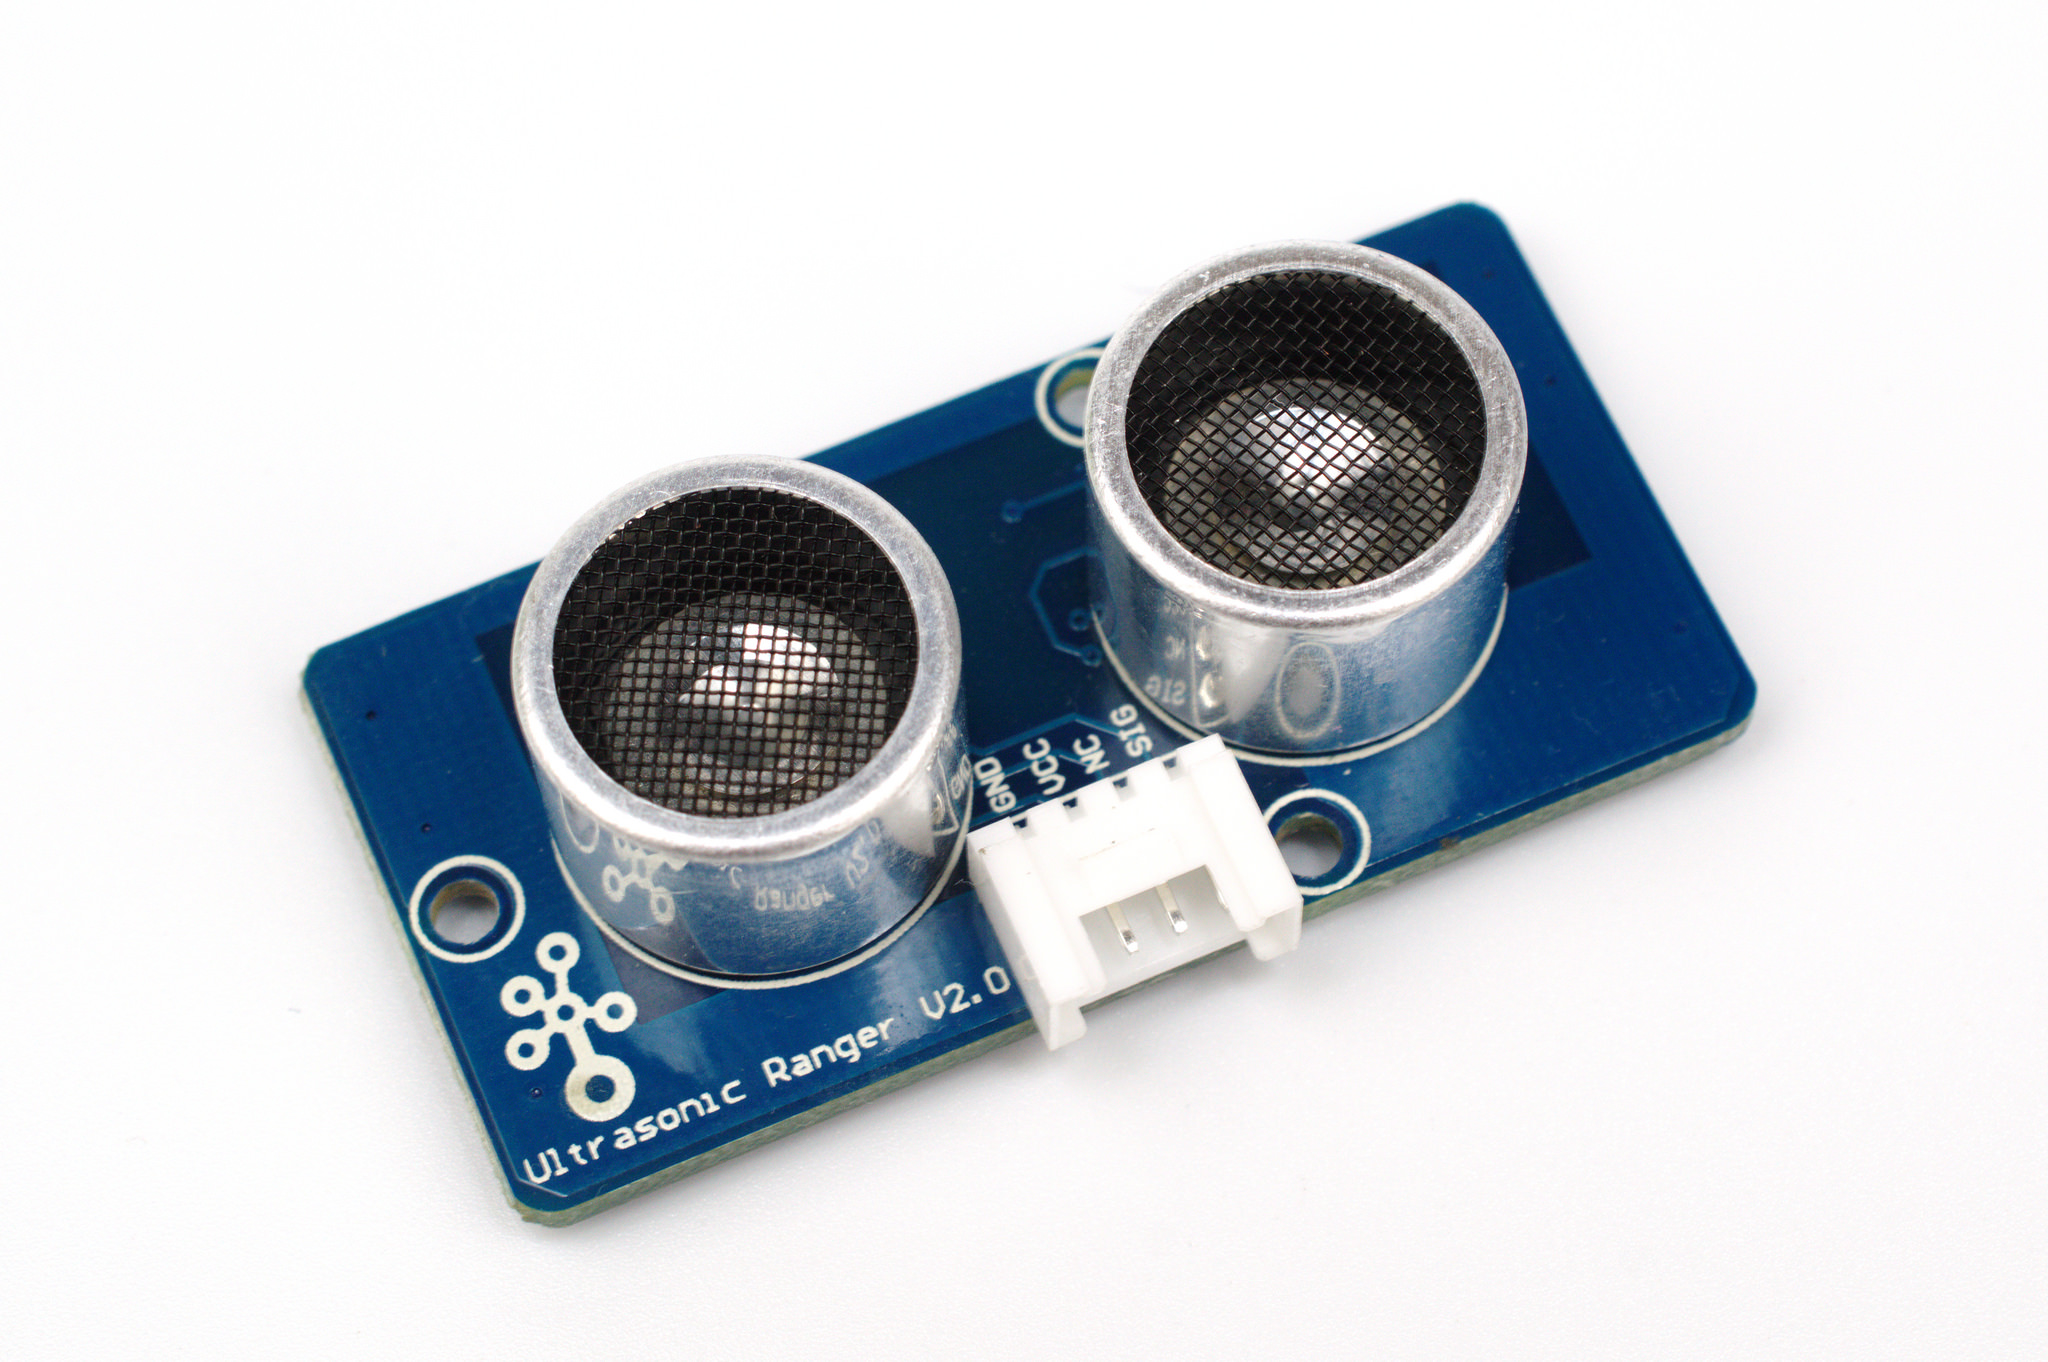
\includegraphics[width=0.2\linewidth, left]{ultrasonic.jpg}
    \end{figure}
    \item Reflective object sensor
    \begin{figure}
        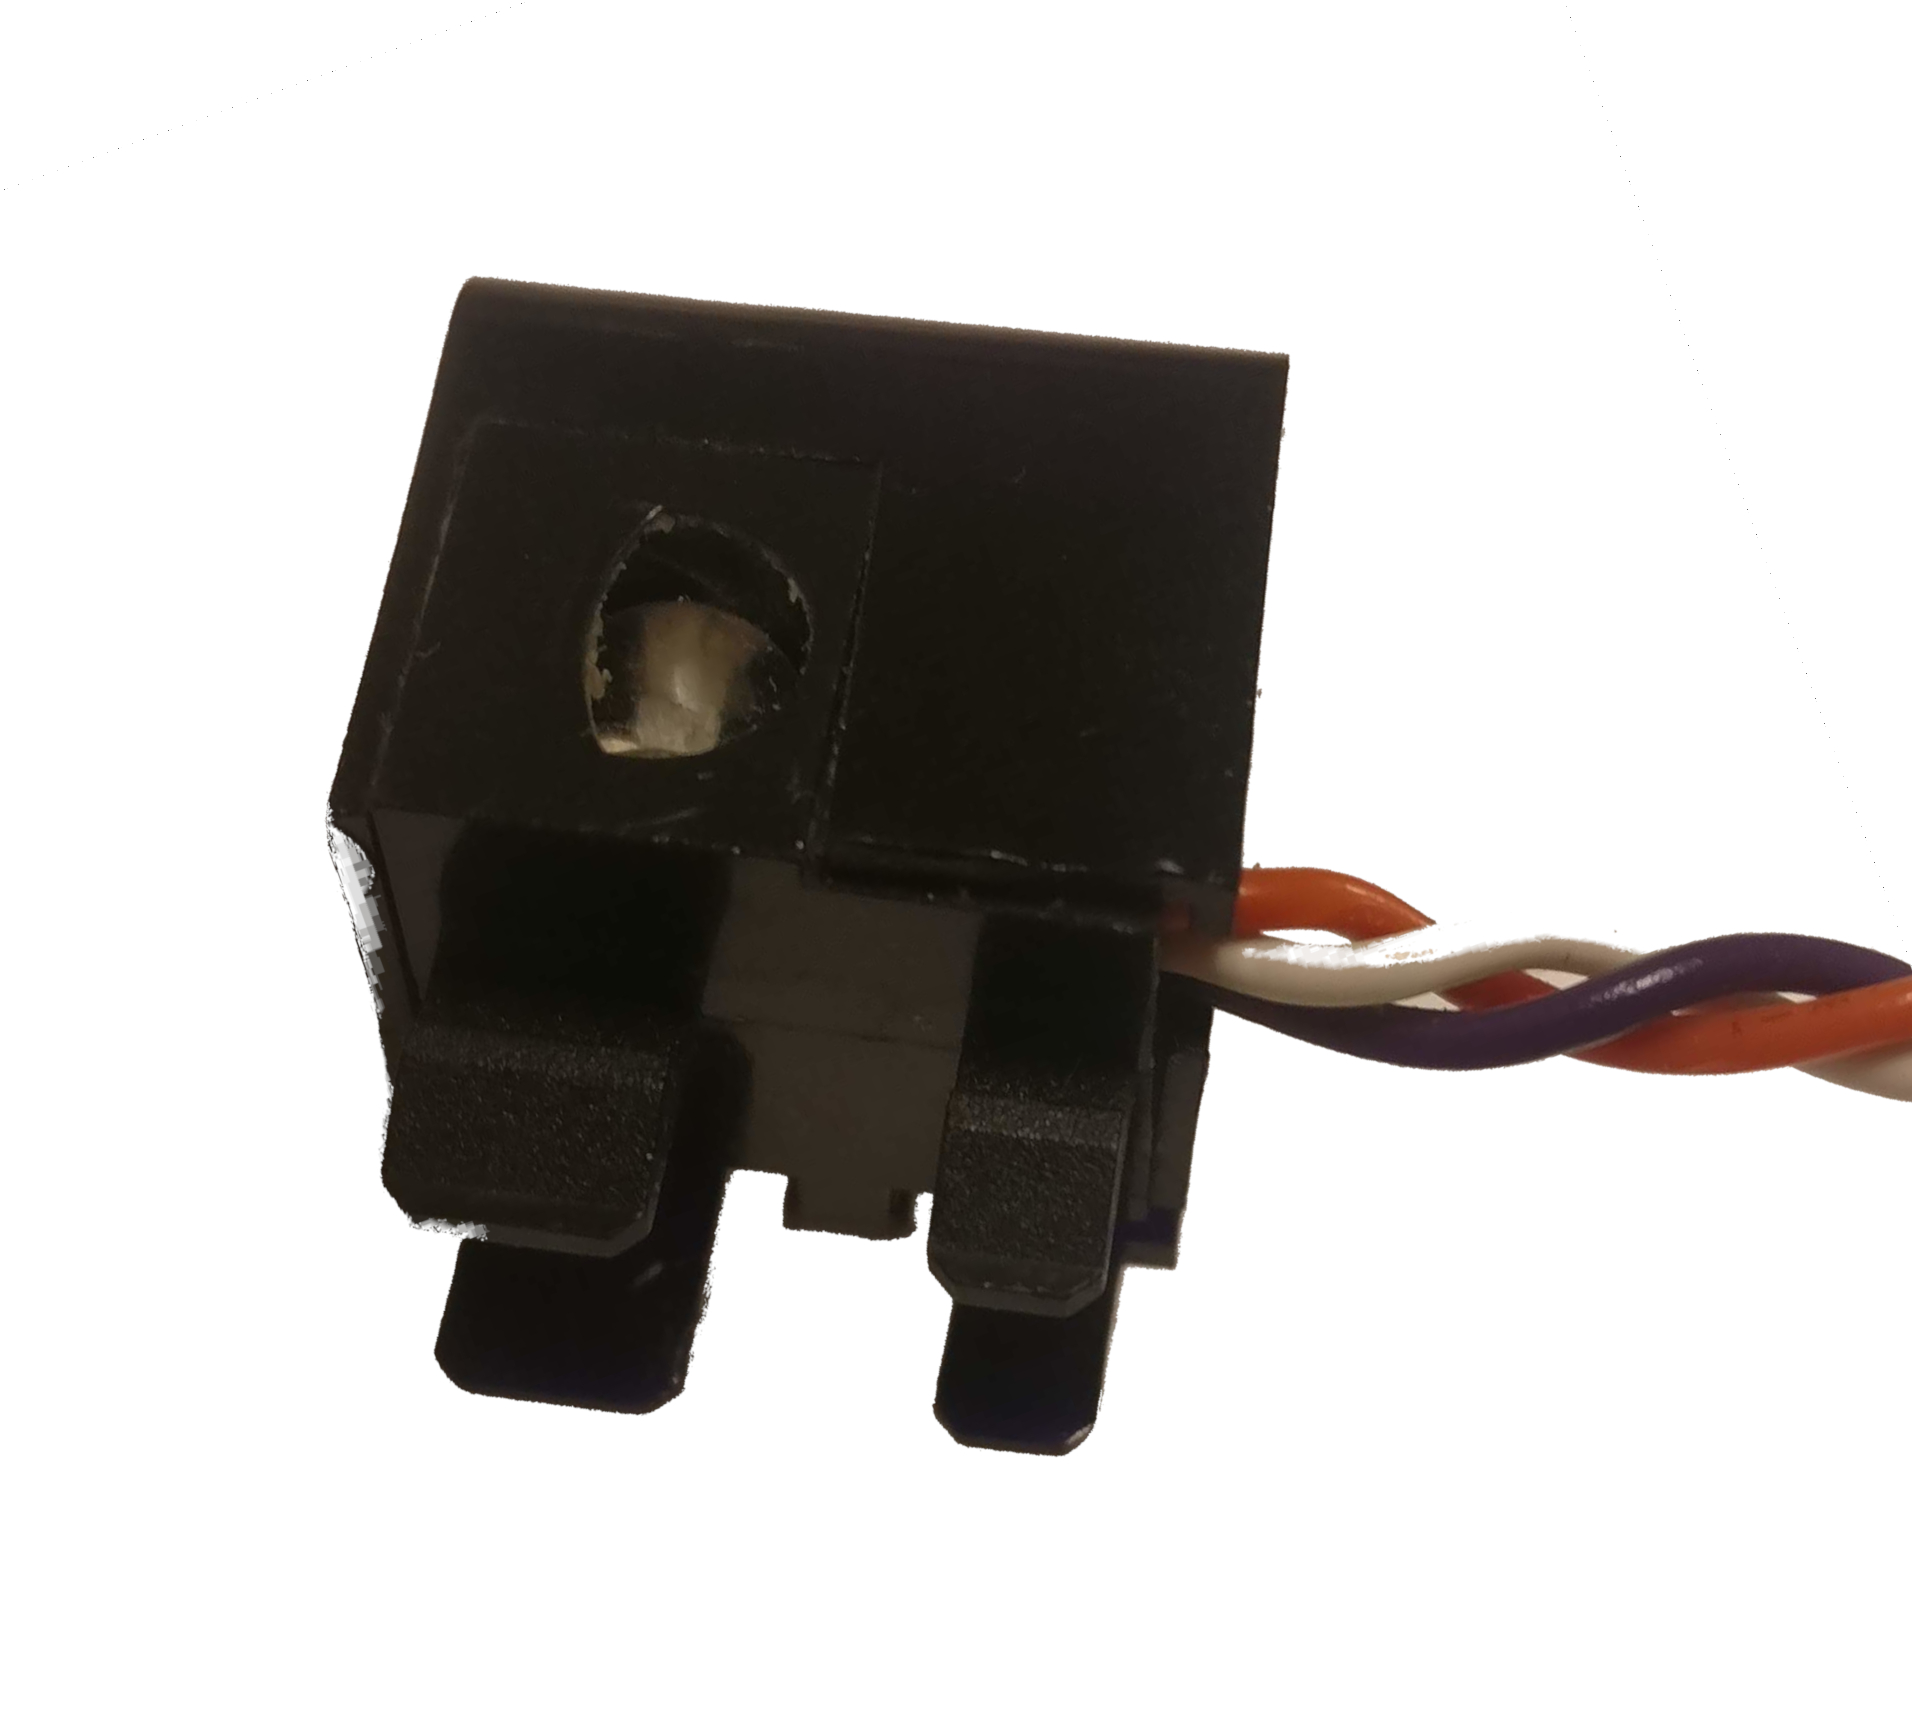
\includegraphics[width=0.2\linewidth, left]{ir.jpg}
    \end{figure}
    \item Camera
    \begin{figure}
        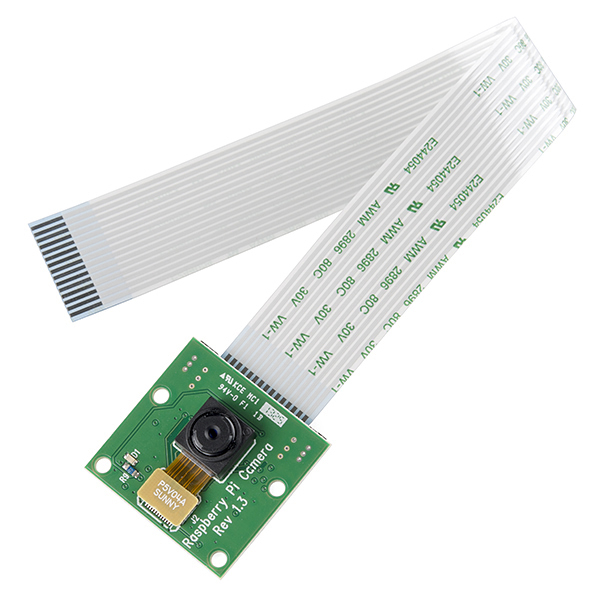
\includegraphics[width=0.2\linewidth, left]{camera.jpg}
    \end{figure}

    \end{itemize}

\end{frame}

%------------------------------------------------

\subsection{Actutators}
\begin{frame}{Actuators}
 \begin{itemize}
  \item Motor controller
  \item Steering controller
 \end{itemize}

\end{frame}

\section{Assembly}
\subsection{Mounting}
\begin{frame}{The platform}
    
    \begin{columns}
        \begin{column}{0.47\textwidth}
            \begin{itemize}
                \item  Designed in Fusion 360
                \item  Cut out in the laser cutter
                \item  The ide of the design was to build up to get access to everything and to be modular
                \item Mounted on the car via two holes 
            \end{itemize}
        \end{column}
        \begin{column}{0.5\textwidth}
            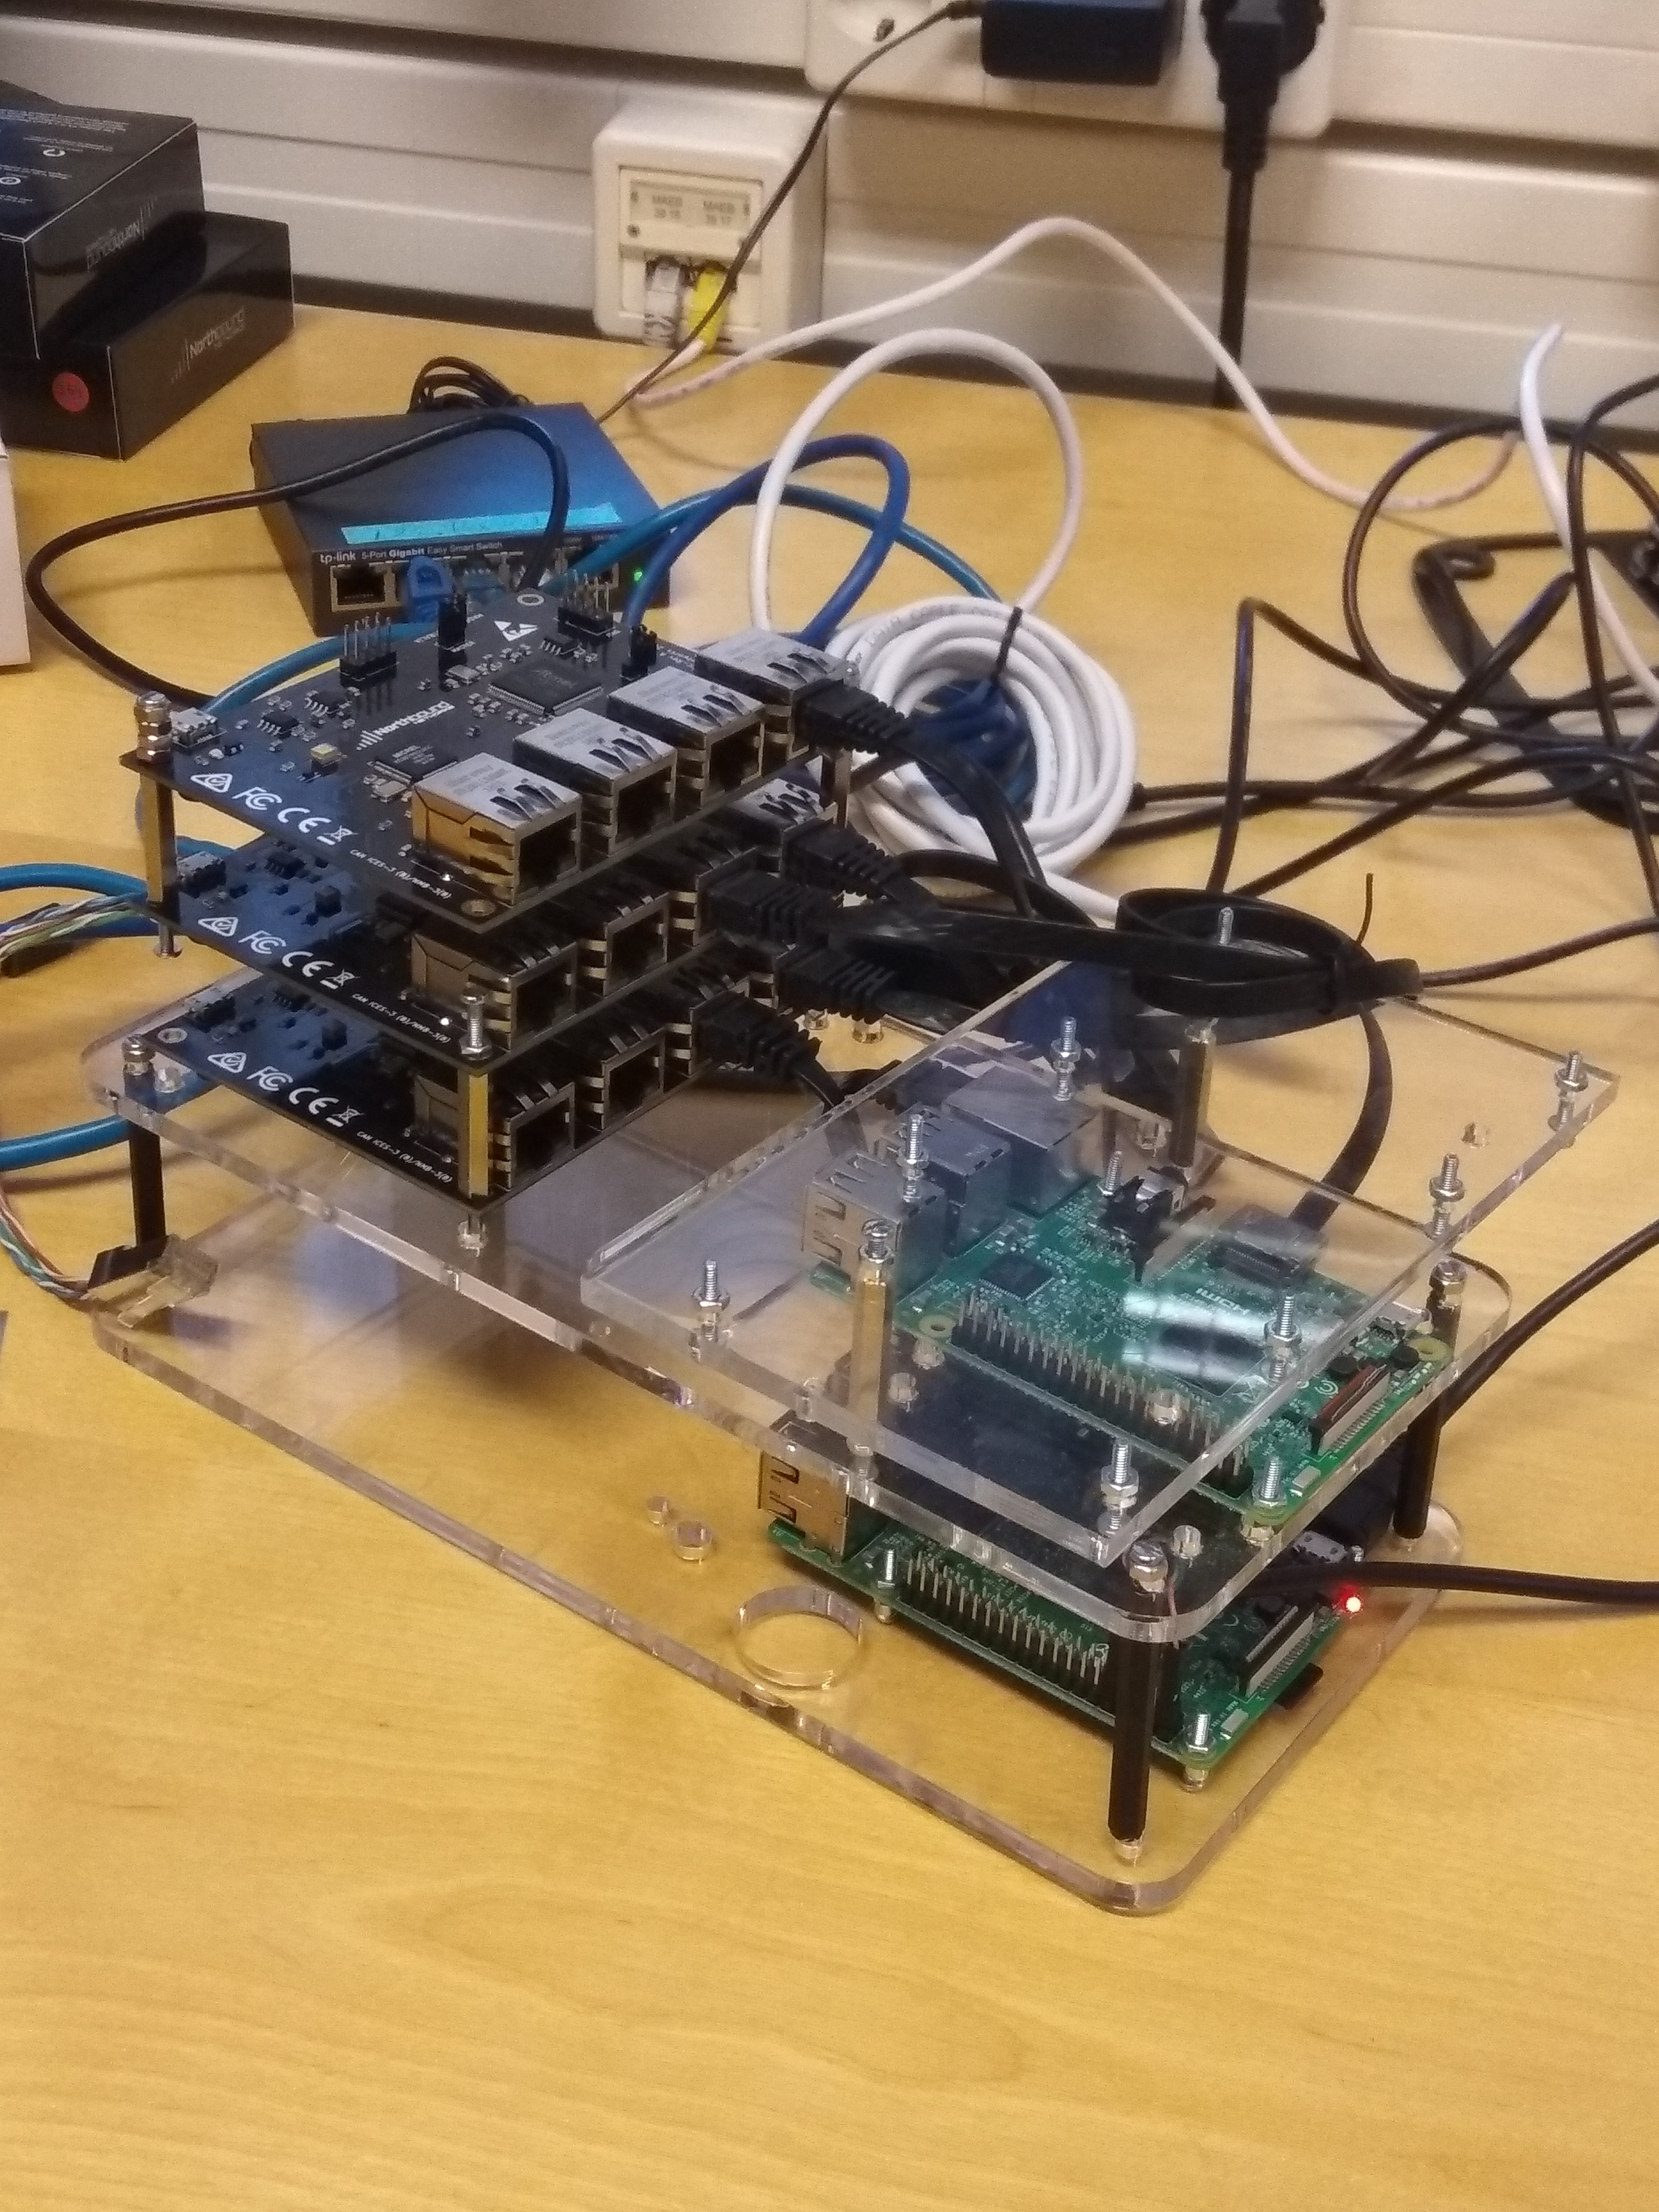
\includegraphics[width=0.7\linewidth]{platform.jpg}
            \label{fig:platform}
            %\caption{Platform}
        \end{column}
    \end{columns}
\end{frame}
\subsection{Power}
\begin{frame}{Power}
    \begin{itemize}
        \item We hade designed PCBs to mount the Arduinos on and to power the other devices
        \item Could not order PCB
        \item The machine PCB mill was broken both the one Mentorspace and proto Prototype Center
        \item Had to use breadboard 
    \end{itemize}
\end{frame}


%------------------------------------------------

\subsection{Autonomous behaviour}
\begin{frame}{Autonomous behaviour}
 \begin{itemize}
  \item Services
  \item State machine
  \begin{figure}
    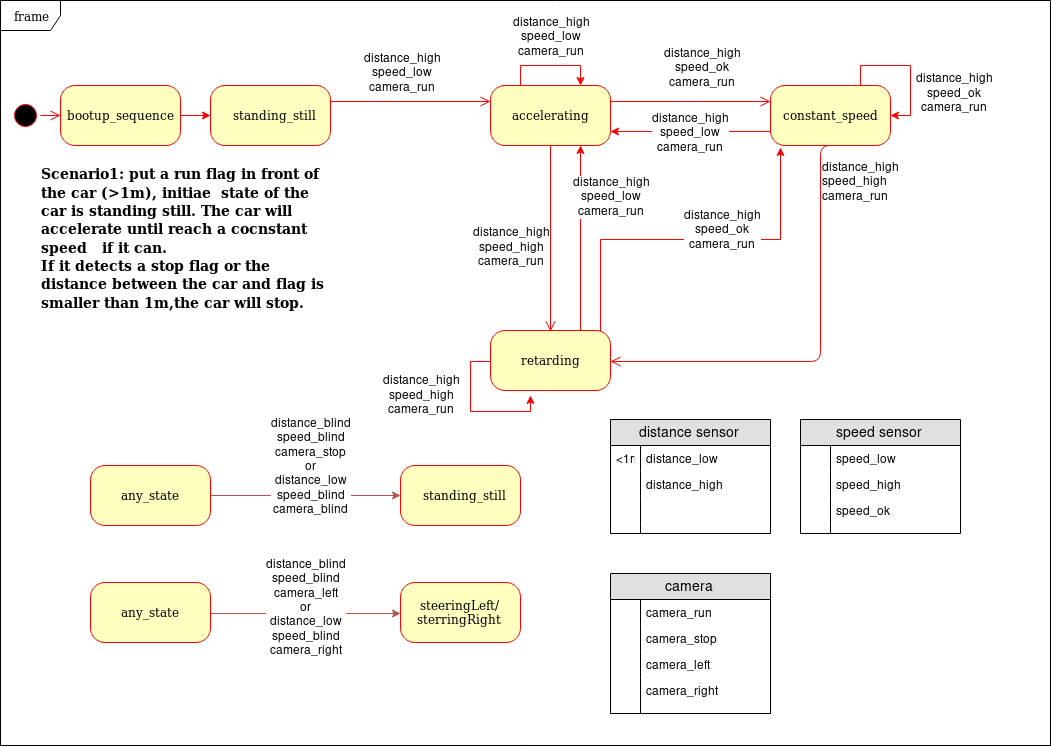
\includegraphics[width=0.7\linewidth]{statemachine.png}
    \caption{State machine}
  \end{figure}
 \end{itemize}

\end{frame}

\section{Assembly}
\subsection{Power}
\subsection{Mounting}

%------------------------------------------------

\section{Conclusion}
\begin{frame}{Conclusion}
    \begin{itemize}
        \item Ethernet is a promising candidate for increasing demand on bandwidth for communication in autonomous cars.
        \item Ethernet is not without problems, which of many SDN is a promising candidate to solve.
        \item SDN networks allow for safe, fast and customisable communication on autonomous vehicles.
        \item Thanks to our project owners! 
    \end{itemize}
    
\end{frame}


%------------------------------------------------


%\begin{frame}
%\frametitle{References}
%\footnotesize{
%\begin{thebibliography}{99} % Beamer does not support BibTeX so %references must be inserted manually as below
%\bibitem[Smith, 2012]{p1} John Smith (2012)
%\newblock Title of the publication
%\newblock \emph{Journal Name} 12(3), 45 -- 678.
%\end{thebibliography}
%}
%\end{frame}

%------------------------------------------------

\begin{frame}
\Huge{\centerline{The End}}
\end{frame}

%----------------------------------------------------------------------------------------

\end{document}
